\documentclass[../root]{subfiles}
\graphicspath{{_images/}{../_images/}}

\begin{document}

    \chapter{Motivating agents: How much does the mission matter?}

    \begin{shortsummary}
        \begin{itemize}
            \item \authoryear{Carpenter2016}
            \item \RQ{How much more productive are workers who believe in the organization’s mission and who are incentivized by monetary reward?}
            \item \answer{Lab experiment of Real Effort Task}
            \item \result{(i) Missions and incentives have strong effects on worker productivity; (ii) incentives have differential effects depending on whether a worker is well matched or not.}
        \end{itemize}
    \end{shortsummary}

    \section{Introduction}

    \begin{figure}[h]
        \centering
        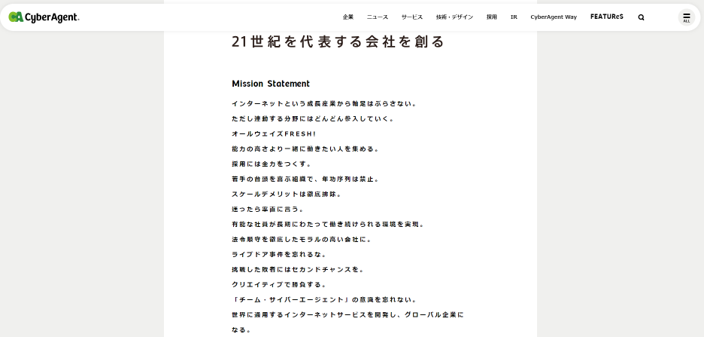
\includegraphics[width = 1.0\linewidth]{os0602kato/eg_cyberagent.PNG}
        \caption{Example of Mission Statement (CyberAgent)}
        \label{Real World Example}
    \end{figure}

    \begin{itemize}
        \item Mission Statements: A way to attract workers whose enthusiasm for the mission translates into higher job satisfaction and greater effort (Evidence from Gallup Survey).
        \item Besley and Ghatak (2005, AER): Financial and mission preferences are substitutes when workers are matched to organizations with which they share a common mission (This is theoretical result).
        \item They have two research questions:
        \begin{enumerate}
            \item Controlling for sorting, exactly how much more productive are workers who believe in the organization’s mission?
            \item In the case of mismatches, can increases in traditional financial incentives make up for the motivational deficit? If pay is based on performance, will even “mismatched” employees work hard?
        \end{enumerate}
        \item What this paper did: A real-effort lab experiment to identify the effects of missions on worker productivity and to examine the extent to which missions and financial incentives are substitutes when motivating workers.
        \item What this paper found: (i) Missions and incentives have strong effects on worker productivity; (ii) Incentives have differential effects depending on whether a worker is well matched or not. For matched workers, piece rates increased productivity by a 13\%. For unmatched workers, piece rates induce an 86\% increase in output
    \end{itemize}

    \section{Theoretical Framework}

    Agent's utility function is given by 
    \begin{align*}
        U(e) = (w + pe) + \theta M(e, \gamma) - C(e), 
    \end{align*}
    where $e$ is continuous effort level, $w$ is fixed payment, $p$ is piece rate wage, 
    and $C(e)$ is convex cost function for effort.

    The second term is the mission preference. 
    $\theta = \{-1,1\}$ indicates whether an agent's motivation is matched with a principal's one $(\theta = 1)$ or not $(\theta = -1)$.
    The parameter $\gamma$ represents the intensity for mission preference.
    Assume that $M(e,0) = 0$ and $M_{e\gamma} > 0$.

    First-order condition is given by $p + \theta M_e = C'(e)$.
    Given this, we have the following three predictions
    \begin{enumerate}
        \item For any offered contract, an agent exerts greater effort when matched compared to when unmatched: $e^*_{\theta = 1} > e^*_{\theta = -1}$.
        \item Incentives will have a stronger effect on the effort of mismatched agents: $de^*_{\theta = -1}/dp > de^*_{\theta = 1}/dp$.
        \item For matches, greater intensity leads to greater effort, while the opposite is the case for mismatches: $de^*_{\theta = -1}/d\gamma < 0$ and $de^*_{\theta = 1}/d\gamma > 0$.
    \end{enumerate}


    \section{Experimental Procedure}

    2x2 between-subject experiment piggybacked on the 2012 political election in the US.
    
    \begin{figure}[h]
        \centering
        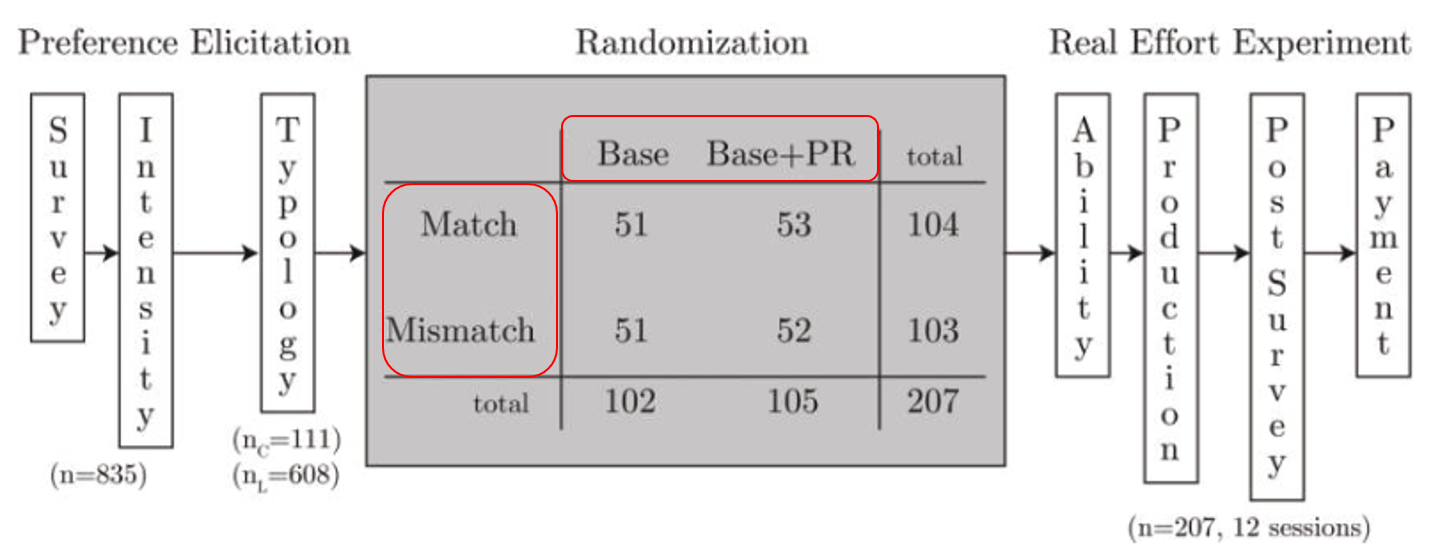
\includegraphics[width = 1.0\linewidth]{os0602kato/exp_proceed.PNG}
        \caption{Experimental Procedure}
        \label{Procedure}
    \end{figure}

    \subsection{Preference Elicitation}

    \begin{figure}[h]
        \centering
        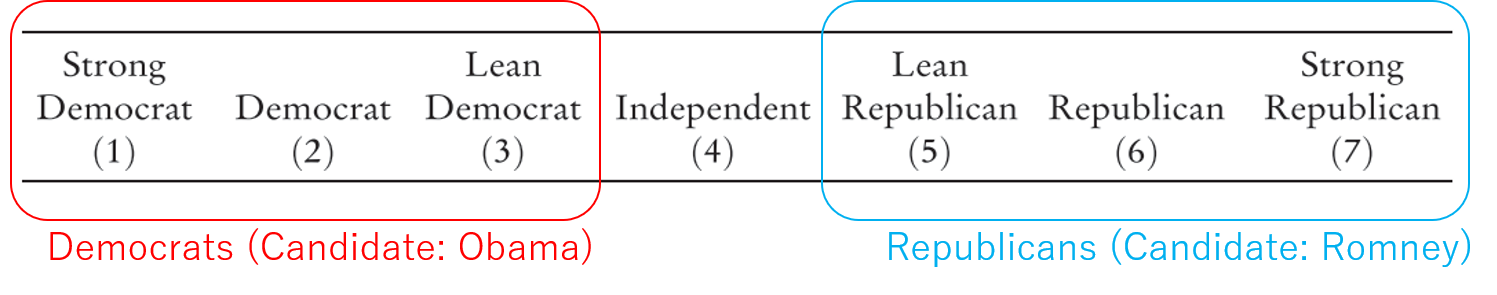
\includegraphics[width = 1.0\linewidth]{os0602kato/poli_preference.PNG}
        \caption{Survey of Political Preference}
        \label{Preference}
    \end{figure}
  
    \begin{itemize}
        \item "Survey" section: elicit political preference (figure \ref{Preference})
        \item "Intensity": Respondents were given \$100 that they could split with the campaign of a major party candidate they had chosen beforehand (Dictator Game).
        \item Study participants work for either the Obama campaign or the Romney campaign (random assignment).
    \end{itemize}

    \subsection{Real Effort Experiment}
    
    \begin{itemize}
        \item Real effort experiment: a letter-stuffing
        \begin{itemize}
            \item "Ability" round: fund-raising letters (all participants)
            \item "Production" round: campaign letters for Obama or Romney
        \end{itemize}
        \item Financial incentives:
        \begin{itemize}
            \item Base: \$20 for 15 minutes of production
            \item Base + PR: Base + a piece rate of \$0.50 (or \$1.00) per completed letter
        \end{itemize}
        \item Remark: Participants are asked to address and stuff letters for the college without compensation.
    \end{itemize}
    
    \subsection{Distribution of Political Preference and Its Intensity}

    \begin{figure}[h]
        \centering
        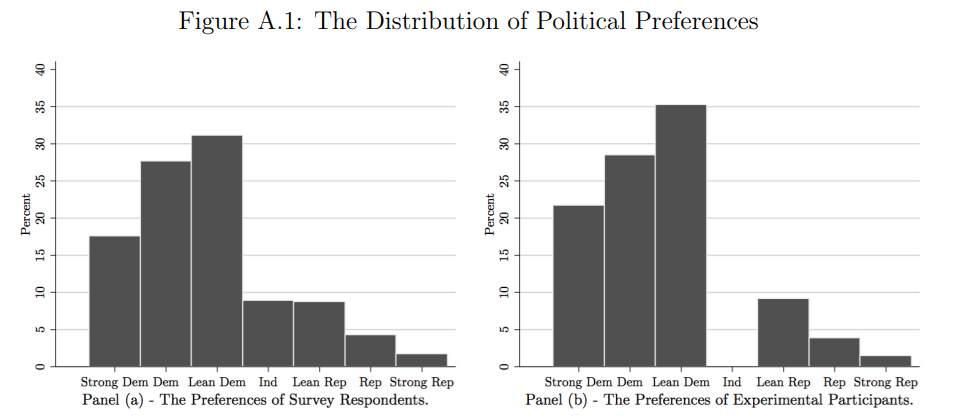
\includegraphics[width = 1.0\linewidth]{os0602kato/pref_result.PNG}
        %\caption{Survey of Political Preference}
        \label{Result: Preference}
    \end{figure}

    \begin{figure}[h]
        \centering
        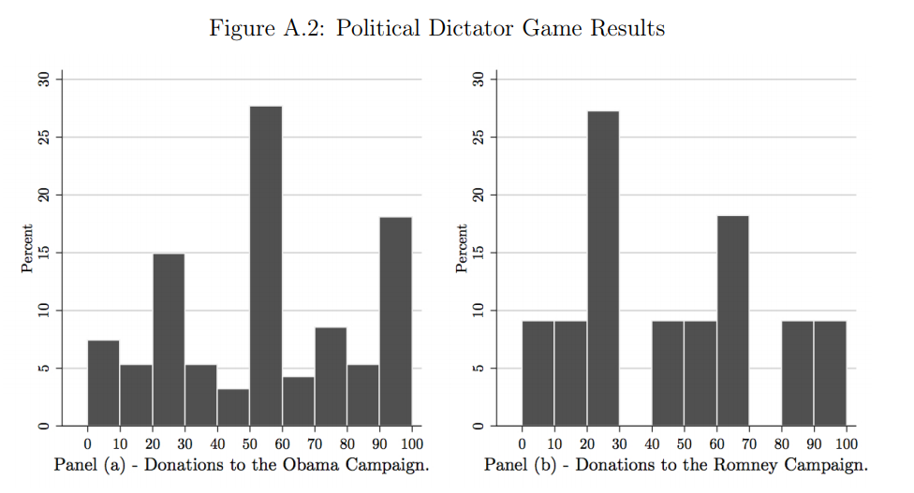
\includegraphics[width = 1.0\linewidth]{os0602kato/intensity_result.PNG}
        %\caption{Survey of Political Preference}
        \label{Result: Intensity}
    \end{figure}


    \section{Results}

    \subsection{Effect of Incentive and Mission}

    \begin{figure}[h]
        \centering
        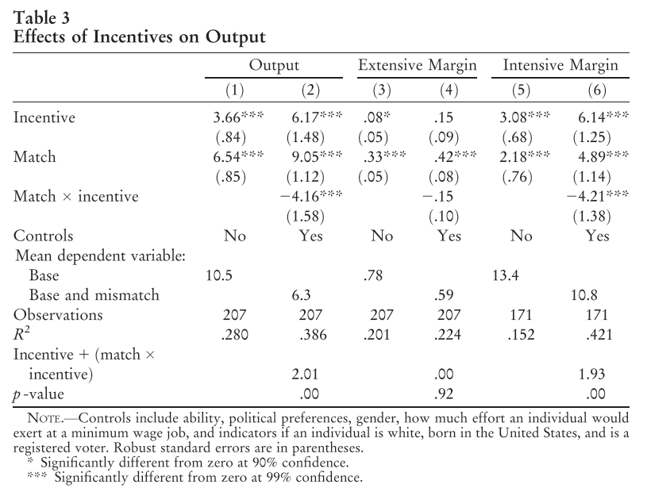
\includegraphics[width = 0.8\linewidth]{os0602kato/reg1.PNG}
        %\caption{Survey of Political Preference}
        \label{Result: Regression 1}
    \end{figure}

    \begin{figure}[h]
        \centering
        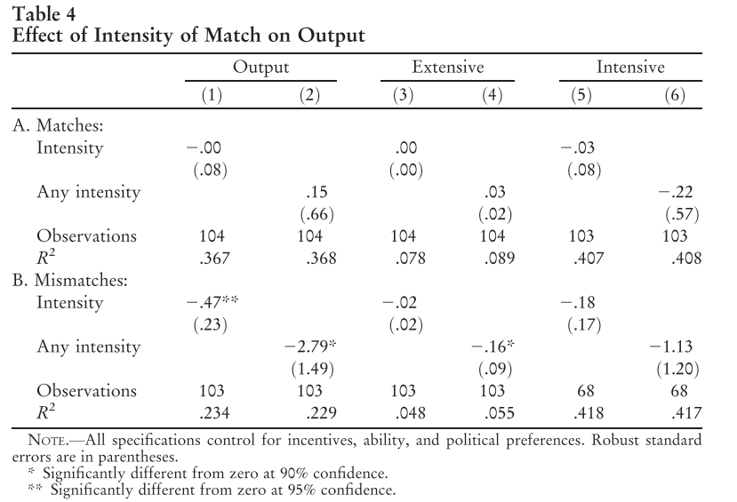
\includegraphics[width = 0.8\linewidth]{os0602kato/reg2.PNG}
        %\caption{Survey of Political Preference}
        \label{Result: Regression 2}
    \end{figure}

    \begin{itemize}
        \item Matching and incentives have positive effects on productivity.
        \item Matching generates larger productivity gains than incentives.
        \item Incentive has little effect on an extensive margin, but a large impact on an intensive margin.
        \item About the intensive margin, the effect of incentives is weaker among the matches than the mismatches.
        \item For the mismatches, greater intensity leads to lower output. On the other hand, for the matches, intensity does not affect output.
    \end{itemize}


    \clearpage
    \subsection{Robustness Check}

    \begin{figure}[h]
        \centering
        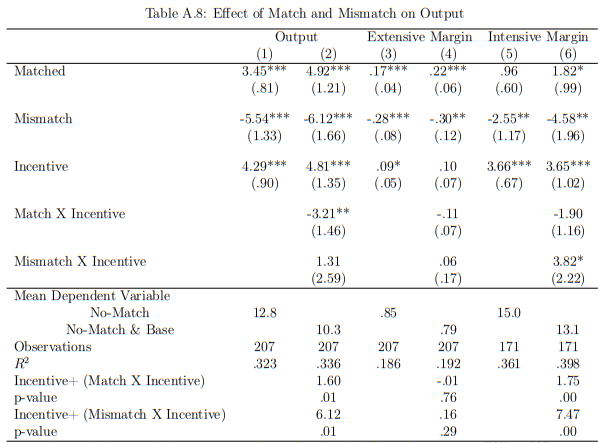
\includegraphics[width = 0.8\linewidth]{os0602kato/reg3.PNG}
        %\caption{Survey of Political Preference}
        \label{Result: Regression 3}
    \end{figure}

    \begin{itemize}
        \item Estimates are upper-biased since authors compare matches to mismatches, not to workers without mission preferences, that is, "no-matches."
        \begin{itemize}
            \item In fact, previous studies shows smaller effects 
        \end{itemize}
        \item Participants who contributed nothing to either candidate are seen as "no-matches." These types have either no or very weak preferences for missions.
        \item Result: The matches increase output rather than the no-matches. The mismatches decrease output rather than the no-matches. Incentive has strong effect among the no-matches.
    \end{itemize}

    \section{Concluding Remarks}

    \begin{quote}
        Not only are your workers likely to be content and productive, potentially costly, high-powered incentives are probably not necessary. If screening on the mission is not possible for the organization, our results suggest that high-powered incentives can overcome much of the motivational deficit caused by poor matches and that incentives do not appear to harm the motivation of workers who are well matched.
    \end{quote}



    \biblio

\end{document}